\chapter{Практическое применение AFL++} \label{ch4}
Рассмотрим процесс фаззинга на практике. В качестве объекта тестирования будет использоваться программа Fuzzgoat(https://github.com/fuzzstati0n/fuzzgoat).
Данное приложение на языке C содержит преднамеренно введенные уязвимости для анализа эффективности фаззеров и инструментов статического анализа.
\section{Фаззинг-тестирование} \label{ch4:sec1}

Перед началом тестирования следует установить инструмент фаззинга AFL++, что предполагает скачивание и компиляцию исходного кода AFL с последующей установкой.

После установки AFL можно приступать к сборке Fuzzgoat с использованием make, при условии, что afl-gcc находится в PATH.

Запуск фаззинга осуществляется командой:
\begin{verbatim}
	afl-fuzz -i in -o out ./fuzzgoat @@
\end{verbatim}

Где:
\begin{itemize}
	\item \texttt{-i in} указывает на директорию с начальными тестами.
	\item \texttt{-o out} обозначает директорию для сохранения результатов фаззинга.
	\item \texttt{./fuzzgoat} — исполняемый файл тестируемой программы.
	\item \texttt{@@} — местозаполнитель, который AFL заменяет на имена файлов из тестового набора.
\end{itemize}

Результаты фаззинга, такие как количество проведенных тестов, скорость тестирования и найденные краши, можно наблюдать в реальном времени в пользовательском интерфейсе AFL. Все найденные ошибки будут сохранены в директорию out/default/crashes.

На \firef{fig:fuzz-panel-ch4} представлена панель мониторинга фаззинг-тестирования.

\begin{figure}[ht] 
	\center
	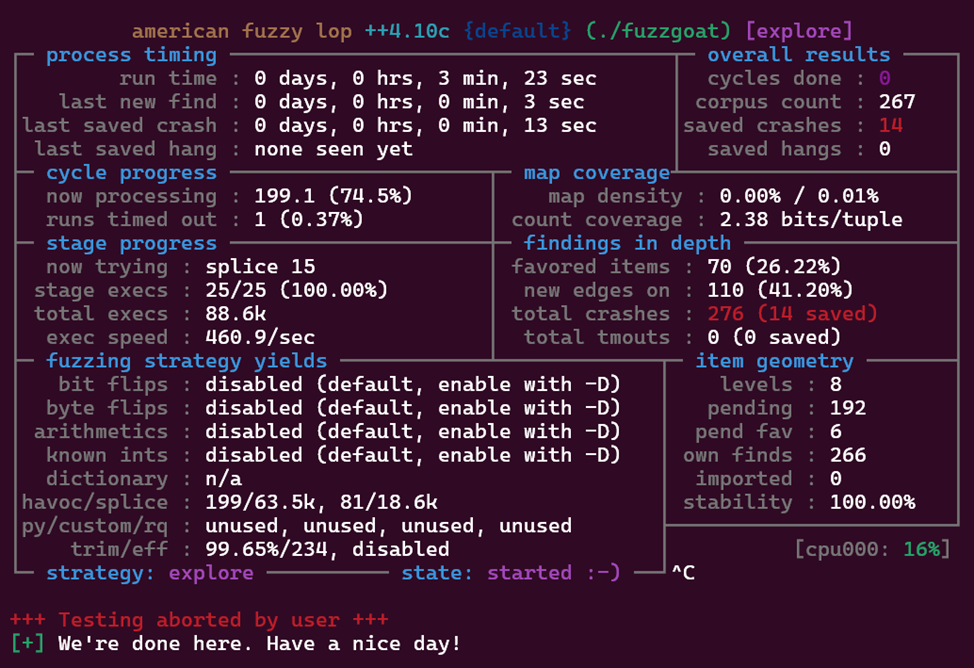
\includegraphics [scale=1] {my_folder/images/fuzz_panel}
	\caption{Панель мониторинга фаззинг-тестирования} 
	\label{fig:fuzz-panel-ch4}  
\end{figure}

На этой панели отображаются результаты процесса тестирования (\firef{fig:overall-res-ch4}).

\begin{figure}[ht] 
	\center
	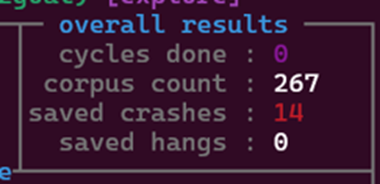
\includegraphics [scale=1] {my_folder/images/overall_res}
	\caption{Текущие результаты фаззинг-тестирования} 
	\label{fig:overall-res-ch4}  
\end{figure}

\begin{itemize}
	\item \textbf{cycles done:} Это количество полных циклов фаззинга, которое было выполнено. Один цикл обычно представляет собой полное исполнение всех тестов в корпусе данных (наборе уникальных тестовых случаев).
	\item \textbf{corpus count:} Количество уникальных тестов, которые в данный момент находятся в "корпусе" — наборе данных для тестирования. AFL++ использует этот корпус как исходный материал для генерации новых входных данных.
	\item \textbf{saved crashes:} Количество уникальных сбоев, которые были обнаружены.
	\item \textbf{saved hangs:} Количество случаев, когда тестируемая программа "зависала" или не отвечала в течение определенного времени, установленного AFL++.
\end{itemize}


\section{Анализ выявленных ошибок} \label{ch4:sec2}
В процессе фаззинга были обнаружены следующие ошибки (\firef{fig:errors-ch4}):

\begin{figure}[ht] 
	\center
	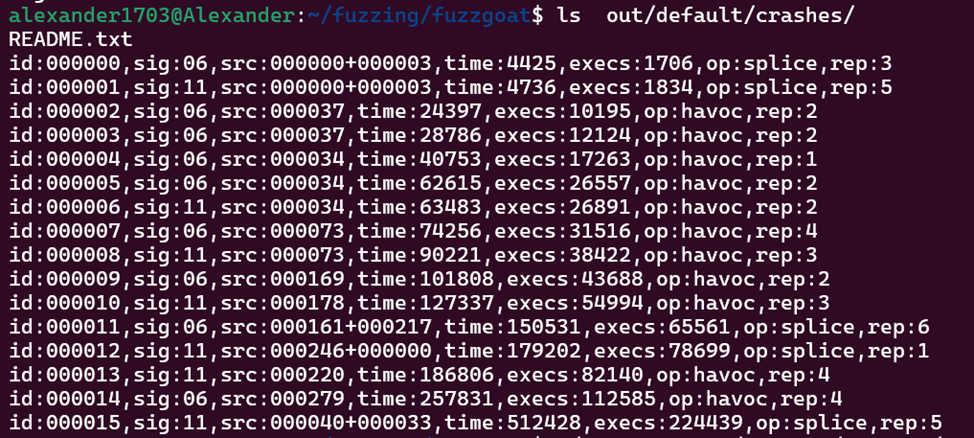
\includegraphics [scale=1] {my_folder/images/errors}
	\caption{Ошибки, выявленные в результате тестирования} 
	\label{fig:errors-ch4}  
\end{figure}

Рассмотрим как AFL именует файлы с ошибками:
id:000015,sig:11,src:000040+000033,time:512428,execs:224439,op:splice,rep:5

\begin{itemize}
	\item \textbf{id:000015:} Это уникальный идентификатор ошибки.
	\item \textbf{sig:11:} Это номер сигнала, который был сгенерирован операционной системой при краше. Сигнал 11 в UNIX-подобных системах — это SIGSEGV, который означает нарушение доступа к памяти (segmentation fault).
	\item \textbf{src:000040+000033:} Это идентификаторы тестовых кейсов из корпуса, которые были использованы для генерации текущего входного файла. В данном случае файл был получен в результате "склеивания" (splice) двух входных файлов с идентификаторами 40 и 33.
	\item \textbf{time:512428:} Время в микросекундах, которое прошло с начала фаззинга до момента обнаружения данной ошибки.
	\item \textbf{execs:224439:} Количество выполнений (исполнений тестов), которое было произведено до обнаружения этой ошибки.
	\item \textbf{op:splice:} Операция, которая была применена к входному файлу, в данном случае "splice" означает, что AFL++ взял части из двух разных файлов корпуса и соединил их вместе, чтобы создать новый тестовый кейс.
	\item \textbf{rep:5:} Количество повторов (репликаций) данной операции, прежде чем был обнаружен краш. Это может означать, что ошибка возникла не с первого раза, а после нескольких попыток с различными мутациями.
\end{itemize}

Чтобы подробнее узнать о найденных ошибках нужно ввести команду
\begin{verbatim}
	./fuzzgoat out/default/crashes/id:000011,...
\end{verbatim}
Где:
\begin{itemize}
	\item ./fuzzgoat — исполняемый файл тестируемой программы
	\item out/default/crashes/id:000011,... - путь до файла
\end{itemize}

Рассмотрим некоторые из ошибок, которые были найдены (\firef{fig:errors-concrete-ch4}):
\begin{figure}[ht] 
	\center
	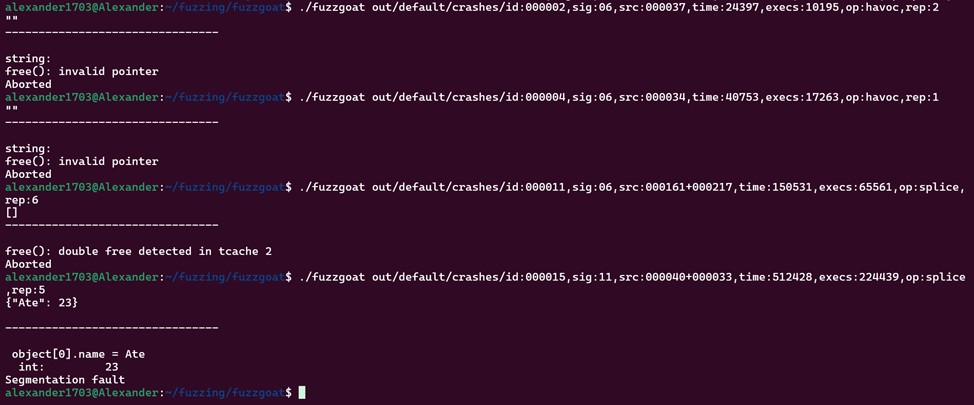
\includegraphics [scale=1] {my_folder/images/errors_concrete}
	\caption{Информация об ошибках, выявленных в процессе тестирования} 
	\label{fig:errors-concrete-ch4}  
\end{figure}

\textbf{free(): invalid pointer}

Попытка освободить память, которая не была выделена через malloc() или аналогичные функции, или уже была освобождена ранее. В данном случае, такая ошибка произошла дважды (id:000002 и id:000004)

\textbf{free(): double free detected in tcache 2}

Программа пытается освободить ту же область памяти более одного раза. 
Ошибка произошла при тесте с id:000011, что показывает, что определенные входные данные приводят к повторному освобождению уже освобожденной памяти.

\textbf{Segmentation fault}

Ошибка доступа к памяти вне выделенного сегмента. Обычно возникает, когда программа пытается читать или писать в память, к которой у нее нет доступа, или когда указатель на память не инициализирован.
Ошибка обнаружена при тестировании с id:000015.


К сожалению, точное место ошибки AFL не возвращает. AFL работает с уже скомпилированным кодом и не имеет прямого доступа к исходному коду программы, что делает невозможным указание точной строки или функции, где произошла ошибка. Фаззер отслеживает лишь факт возникновения сбоя, без анализа причин его возникновения на уровне исходного кода. Для определения конкретной причины и места сбоя необходимо использовать дополнительные инструменты, например профилировщики.

% не рекомендуется использовать отдельную section <<введение>> после лета 2020 года
%\section{Введение} \label{ch4:intro}

%Хорошим стилем является наличие введения к главе. Во введении может быть описана цель написания главы, а также приведена краткая структура главы. 
%	
%\section{Название параграфа} \label{ch4:sec1}
%
%\section{Название параграфа} \label{ch4:sec2}
%
%Пример ссылки на литературу \cite{avtonomova:fya,Peskov2004-ru,Kotelnikov2004-ru,Kotelnikov2004}.
%
%%\FloatBarrier % заставить рисунки и другие подвижные (float) элементы остановиться
%
%\section{Выводы} \label{ch4:conclusion}
%
%Текст выводов по главе \thechapter.

%% Вспомогательные команды - Additional commands
%
%\newpage % принудительное начало с новой страницы, использовать только в конце раздела
%\clearpage % осуществляется пакетом <<placeins>> в пределах секций
%\newpage\leavevmode\thispagestyle{empty}\newpage % 100 % начало новой страницы